% Template for Cogsci submission with R Markdown

% Stuff changed from original Markdown PLOS Template
\documentclass[10pt, letterpaper]{article}

\usepackage{cogsci}
\usepackage{pslatex}
\usepackage{float}
\usepackage{caption}

% amsmath package, useful for mathematical formulas
\usepackage{amsmath}

% amssymb package, useful for mathematical symbols
\usepackage{amssymb}

% hyperref package, useful for hyperlinks
\usepackage{hyperref}

% graphicx package, useful for including eps and pdf graphics
% include graphics with the command \includegraphics
\usepackage{graphicx}

% Sweave(-like)
\usepackage{fancyvrb}
\DefineVerbatimEnvironment{Sinput}{Verbatim}{fontshape=sl}
\DefineVerbatimEnvironment{Soutput}{Verbatim}{}
\DefineVerbatimEnvironment{Scode}{Verbatim}{fontshape=sl}
\newenvironment{Schunk}{}{}
\DefineVerbatimEnvironment{Code}{Verbatim}{}
\DefineVerbatimEnvironment{CodeInput}{Verbatim}{fontshape=sl}
\DefineVerbatimEnvironment{CodeOutput}{Verbatim}{}
\newenvironment{CodeChunk}{}{}

% cite package, to clean up citations in the main text. Do not remove.
\usepackage{apacite}

% KM added 1/4/18 to allow control of blind submission
\cogscifinalcopy

\usepackage{color}

% Use doublespacing - comment out for single spacing
%\usepackage{setspace}
%\doublespacing


% % Text layout
% \topmargin 0.0cm
% \oddsidemargin 0.5cm
% \evensidemargin 0.5cm
% \textwidth 16cm
% \textheight 21cm

\title{Characterizing Contextual Variation in Children's Preschool
Language Environment Using Naturalistic Egocentric Videos}


\author{{\large \bf Robert Z. Sparks, Bria Long, Grace E. Keene, Malia J. Perez,} \\ {\large \bf Alvin W.M. Tan, Virginia A. Marchman, Michael C. Frank} \\ bsparks@stanford.edu, bria@stanford.edu, gkeene@stanford.edu, mjperez@stanford.edu, \\ tanawm@stanford.edu, marchman@stanford.edu, mcfrank@stanford.edu \\ Department of Psychology, Stanford University}

\newlength{\cslhangindent}
\setlength{\cslhangindent}{1.5em}
%\newenvironment{CSLReferences}%
%  {}%
%  {\par}

\newlength{\csllabelwidth}
\setlength{\csllabelwidth}{3em}
\newlength{\cslentryspacingunit} % times entry-spacing
\setlength{\cslentryspacingunit}{\parskip}

% for Pandoc 2.8 to 2.10.1
\newenvironment{cslreferences}%
{}%
{\par}
% For Pandoc 2.11+
\newenvironment{CSLReferences}[2] % #1 hanging-ident, #2 entry spacing
{% don't indent paragraphs
	\setlength{\parindent}{0pt}
	% turn on hanging indent if param 1 is 1
	\ifodd #1
	\let\oldpar\par
	\def\par{\hangindent=\cslhangindent\oldpar}
	\fi
	% set entry spacing
	%\setlength{\parskip}{#2\cslentryspacingunit}
}%
{}
\usepackage{calc}
\newcommand{\CSLBlock}[1]{#1\hfill\break}
\newcommand{\CSLLeftMargin}[1]{\parbox[t]{\csllabelwidth}{#1}}
\newcommand{\CSLRightInline}[1]{\parbox[t]{\linewidth - \csllabelwidth}{#1}\break}
\newcommand{\CSLIndent}[1]{\hspace{\cslhangindent}#1}


\begin{document}

\maketitle

\begin{abstract}
What structures children's early language environment? Large corpora of
child-centered naturalistic recordings provide an important window into
this question, but most available data centers on young children within
the home or in lab contexts interacting primarily with a single
caregiver. Here, we characterize children's language experience in a
very different kind of environment: the preschool classroom. Children
ages 3 -- 5 years (N = 26) wore a head-mounted camera in their preschool
class, yielding a naturalistic, egocentric view of children's everyday
experience across many classroom activity contexts (e.g., sand play,
snack time), with \textgreater30 hours of video data. Using
semi-automatic transcriptions (227,624 words), we find that activity
contexts in the preschool classroom vary in both the quality and
quantity of the language that children both hear and produce. Together,
these findings reinforce prior theories emphasizing the contribution of
activity contexts in structuring the variability in children's early
learning environments.

\textbf{Keywords:}
Classroom Studies, Head-Mounted Cameras, Language Development,
Naturalistic Recordings
\end{abstract}

\hypertarget{introduction}{%
\section{Introduction}\label{introduction}}

How do children learn language from their everyday experiences?
Children's experiences are highly varied, characterized by both
one-on-one interactions with caregivers, interactions with siblings and
peers, overheard interactions between adults or other children, and many
other contexts. Yet most theories have been developed via observation of
idealized interactions between caregivers and children in experimental
contexts (Aslin, 2007; Bergmann et al., 2018). Acknowledging the
richness of children's home environments, more recent work has made use
of home recordings to characterize the developmental experience of
infants. Daylong audio recordings (Bergelson, Amatuni, Dailey,
Koorathota, \& Tor, 2019; Greenwood, Thiemann-Bourque, Walker, Buzhardt,
\& Gilkerson, 2011; VanDam et al., 2016) and egocentric video recordings
of the home using head-mounted cameras (Aslin, 2009; Smith, Yu, Yoshida,
\& Fausey, 2015; Sullivan, Mei, Perfors, Wojcik, \& Frank, 2021) both
provide insight into understanding everyday learning environments and
show non-uniformity across developmental experience (Barbaro \& Fausey,
2022). Such data highlight the need to unpack the heterogeneity of the
experiences that shape children's development by building more
naturalistic datasets that help to characterize the daylong experiences
of children.

Exploring naturalistic accounts of child experience reveal a multitude
of different spatial, temporal, and activity contexts, which are
associated with correspondingly different language environments. Over
the course of a day, children may eat in the dining area, play with toys
in the living room, take a bath in the bathroom, and interact with other
social partners outside the home. Language input varies across these
activity contexts, in terms of the quantity, lexical diversity, mean
length of utterance, and semantic content of caregivers' speech (Bang,
Mora, Munévar, Fernald, \& Marchman, 2022; Glas, Rossi, Hamdi-Sultan,
Batailler, \& Bellemmouche, 2018; Hoff-Ginsberg, 1991; Tamis-LeMonda,
Custode, Kuchirko, Escobar, \& Lo, 2019). This variation in language
input also has implications for children's language acquisition---for
example, words used in distinctive contexts (e.g., words strongly
associated with the bathroom or kitchen contexts) may be learned earlier
than words used across many contexts (Roy, Frank, DeCamp, Miller, \&
Roy, 2015). As such, it is important to understand and characterize
children's learning environments across different activity contexts to
capture their true language experiences (Casillas, 2023).

However, there is limited work characterizing children's learning
environments across distinct activity contexts outside of the home.
Early childhood educational contexts are especially important for early
language development. Approximately 54\% of preschool-aged children are
enrolled in early childhood education (ECE) globally, with some children
spending up to 40 hours a week in preschools (Raikes et al., 2023).
Evidence supporting the effectiveness of preschool on short-term
developmental processes (language, cognitive, and social outcomes) and
school achievement (Camilli, Vargas, Ryan, \& Barnett, 2010; G. J.
Duncan \& Magnuson, 2013) motivates a need to appropriately describe the
language environments in these ECE contexts.

Earlier work characterizing children's preschool learning environments
has relied heavily on third-person observation (Sawyer et al., 2018).
Video-based observations have largely been limited to full-classroom
views focused on head-teacher speech to all children (Dickinson, Darrow,
\& Tinubu, 2008; Justice, Jiang, \& Strasser, 2018). These macro-level
observations are likely a product of technical limitations. Cumbersome
and invasive recording technology may prevent researchers from capturing
more naturalistic, child-level recordings without being disruptive to
the children or the classroom. Obtaining permission from parents both to
intervene on normal class time and to record in the classroom provides
another potential obstacle to capturing more precise recordings of the
preschool language environment.

A growing body of research has sought to study ECE language environments
using child-centered recordings that capture a more holistic view of the
preschool classroom inclusive of peer-peer interactions. Technical
innovations such as the Language Environment Analysis (LENA) device
(\url{http://www.lenafoundation.org/lena-pro/}) allow for researchers to
capture non-invasive, child-centered audio recordings of children's
environments. Recent work has used this new technology to capture
child-centered audio recordings of the preschool language environment
(R. J. Duncan et al., 2020; R. J. Duncan et al., 2023; Perry et al.,
2018). Other work has built on existing headcam literature by capturing
egocentric video of children's preschool environments (Chaparro-Moreno,
Justice, Logan, Purtell, \& Lin, 2019). In addition, recent research has
introduced higher-resolution headcams with additional sensors, including
gyroscopes and accelerometers, that hold the promise of detailed
characterization of children's behavior in richer, more active play
contexts (Geangu et al., 2023; Long et al., 2022).

Just as the home, the preschool classroom is not a uniform context for
interactions. Studies using daylong-audio and egocentric video in the
preschool classroom demonstrate significant variability in language
environments across time, across classrooms, and across individual
children within classrooms. Other observational studies demonstrate that
early learning in preschool classrooms relies on complex social dynamics
involving many different people and activity types (Booren, Downer, \&
Vitiello, 2012; Sawyer et al., 2018). Related work also suggests that
features of classroom language environments can serve as predictors of
child language outcomes, such as, vocabulary size (R. J. Duncan et al.,
2023; Perry et al., 2018). While prior work has observed variability in
the language environment, the specific contributions of activity
contexts to ECE language environments are not well characterized. Given
that children dynamically shift between many distinct activity contexts
across the day (e.g., story time, meals, arts and crafts), it is
important to characterize the context-specific language environments
that can potentially scaffold early learning in different ways.

In the current work, we use novel video recordings of children's
egocentric perspective to characterize the speech occurring in the
dynamic learning environments of a preschool classroom. We record a wide
range of experiences in the classroom, including self-guided play,
exploration, and interactions both between children, as well as between
children and teachers. In total, we recorded from the perspective of 26
unique children on 13 days over a 4 week period, totaling 30.66 hours of
observation. Using these egocentric recordings, we were able to label
moment-to-moment activity contexts of children as they freely navigated
the preschool classroom. We then evaluated both the quality (Lexical
Diversity, MLU-w, Lexical Complexity, Keyness) and the quantity (Speech
Rate) of the language that children hear and produce. These measures
reveal variability in children's language input and output across
activity contexts. Our findings emphasize a non-uniform preschool
language environment that changes with the activity contexts in which
children engage.

\hypertarget{methods}{%
\section{Methods}\label{methods}}

\hypertarget{participants}{%
\subsection{Participants}\label{participants}}

34 children from a local nursery school classroom at Stanford University
were consented by their parents to be asked to record as a part of this
study. This nursery school is a Montessori-like preschool defined by a
play-based curriculum and self-guided learning. 26 children (2;11-5;11
years, average age = 4.55 years, 50\% male/female, 7.69\% African
American/Black, 19.2\% Asian American/Pacific Islander, 38.5\%
Caucasian/White, 7.69\% Hispanic/Latinx, 30.8\% multiracial, 3.85\%
other) recorded at least one session.

\begin{CodeChunk}
\begin{figure}[ht!]

{\centering 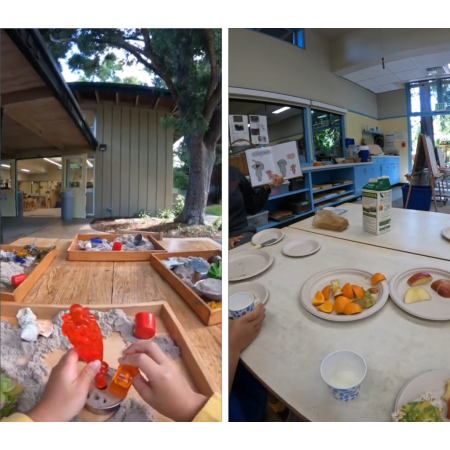
\includegraphics[width=0.75\linewidth]{figs/example-image-1} 

}

\caption[Outdoor (Patio) and indoor (Snack time) child-centered views of the classroom from the BabyView Camera]{Outdoor (Patio) and indoor (Snack time) child-centered views of the classroom from the BabyView Camera.}\label{fig:example-image}
\end{figure}
\end{CodeChunk}

Written consent was provided by one or more parents of each child. A
researcher spoke directly with parents outside of normal classroom hours
to introduce the study and answer questions. Each parent was shown the
camera and given details about how data would be collected and used.
Parents provided consent for recording and broad sharing of the
resulting data. Before each session, children provided verbal assent to
both wear the helmet and make a recording. The child assent process was
also detailed to families, and we made it clear that no child would be
required to wear the helmet or make a recording. Of the 37 children in
the classroom, the parents of three children did not provide consent.
Unconsented children remained in the classroom during recordings, and
researchers worked with teaching staff to provide opportunities for play
away from recordings. Videos were reviewed manually to blackout frames
that included unconsented children and to mute portions of audio
containing speech from an unconsented child. Parents of unconsented
children were made aware of this process before recording began.

\hypertarget{procedure}{%
\subsection{Procedure}\label{procedure}}

Videos from the child's perspective were recorded using an adapted
version of the BabyView camera (Long et al., 2022) (see Figure
\ref{fig:example-image} for examples of this view). This head camera is
a GoPro Hero 10 Bones camera mounted via a 3D printed fixture on a child
safety helmet designed for infants and toddlers. We adjusted the straps
and elastic so that helmets would securely and comfortably fit the heads
of preschoolers. Children were introduced to the camera as the
``Ladybug'' across two class sessions. Children were told that if they
wore the ``Ladybug,'' it would make a movie of their play in the
classroom. Children were approached and asked if they would like to make
a movie, and if they agreed, they confirmed that it was okay to put the
helmet on their head. Children were told that they could make a movie
for as long as they would like and could stop the recording at any time.
Researchers maintained close-distance with the child to allow for
monitoring of the child and their camera, but otherwise avoided
engagement with the child \footnote{Research is conducted frequently at
  this nursery school and researchers are introduced to children as
  additional ``Teachers.'' Thus, having researchers in the classroom is
  normal and children will often approach researchers as teachers during
  regular daily activities.}. We attempted to record a total of 45
minutes with each child, and on any given recording day, researchers
prioritized approaching children who had not yet met this threshold.
Recordings were collected during 13 separate sessions over a 4 week
period. Up to 3 cameras were in use during any given session.

\hypertarget{data}{%
\subsection{Data}\label{data}}

We initially collected 89 individual sessions resulting in 30.66 hours
of recordings. Six sessions were excluded from analyses for being
shorter than 3 minutes. Shorter sessions tended to indicate that the
child wanted to end the session early and resulted in transcripts mostly
involving researcher intervention and child preoccupation with removing
the helmet. Thus, the final sample consisted of 83 sessions yielding a
total of 30.52 hours of video data (3.27-57.82 minutes per session, M =
22.06 minutes). Because children could record during multiple recording
sessions, on average, individual children contributed 73.24 minutes
(range 30.13-116.02 minutes). All materials and code for analysis are
available at \url{https://osf.io/967zv/} (see Figure
\ref{fig:pipeline-image} for overview of analysis pipeline).

\begin{CodeChunk}
\begin{figure}[ht!]

{\centering \includegraphics{figs/pipeline-image-1} 

}

\caption[Overview of the analysis pipeline]{Overview of the analysis pipeline.}\label{fig:pipeline-image}
\end{figure}
\end{CodeChunk}

\hypertarget{transcription}{%
\subsubsection{Transcription}\label{transcription}}

For each video, we extracted the audio data using FFmpeg, and
automatically transcribed the audio using the distil-medium.en model of
Distil-Whisper (Gandhi, Platen, \& Rush, 2023),
\url{https://huggingface.co/distil-whisper/distil-medium.en}, a
distilled version of the Whisper model (Radford et al., 2022). Whisper
is an automatic speech recognition (ASR) model that allows for
transcription of speech audio to text form. While Whisper is generally
accurate for adult speech, its training data included relatively few
datasets of children's speech, especially speech from young children; as
such, Whisper models are likely to be less robust to child speech (Jain,
Barcovschi, Yiwere, Corcoran, \& Cucu, 2023). Preschool classrooms are
also incredibly noisy, with many children and teachers talking
concurrently over ambient noise produced from classroom activities and
the surrounding environments (e.g.~construction).

\hypertarget{transcript-validation}{%
\subsubsection{Transcript validation}\label{transcript-validation}}

To ensure reliability of the produced transcripts for analysis, we
validated a subset of utterances transcribed by ASR. Each session was
divided into video segments of approximately 12 minutes, as a result of
the internal caching mechanism of the GoPro camera. For each video
segment, we extracted the 30 seconds of video beginning at the midpoint
of the video for validation. One of the authors manually annotated the
validation set by watching the corresponding section of the video and
transcribing the speech. We then computed a Word Error Rate (WER) for
the validation set. WER is operationalized as the ratio of the number of
word-level errors to the total number of words in the original
utterance. WER was calculated using the same WER evaluation model used
by Ghandi et. al.~in the evaluation of their Distil-Whisper models
(\url{https://huggingface.co/spaces/evaluate-metric/wer}). Across the
full dataset, a total of 33153 utterances (20490 adult utterances, 12663
child utterances) were semi-automatically transcribed, prior to data
checking and annotation. Of those, a total of 2176 utterances (1298
adult utterances, 877 child utterances, 6.56\% of total utterances) from
149.1 minutes (8.1\% of total recording time) of recordings were
validated. We found WER for the full validation set (14.42\%), corrected
adult utterances (12.31\%), and corrected child utterances (18.41\%).
These results are comparable to long-form evaluation of the
distil-medium.en model (12.4\%).

\hypertarget{annotation-of-speakers-and-activity-contexts}{%
\subsubsection{Annotation of speakers and activity
contexts}\label{annotation-of-speakers-and-activity-contexts}}

Each video was manually reviewed by a researcher who watched the video
alongside the transcript. Video coders assigned a speaker and an
activity context for every transcribed utterance. The speaker of each
utterance was identified as the key child, another child, a teacher, or
a researcher. When the coder identified an utterance that included
speech from more than one speaker, utterances were separated into
multiple utterances and speakers were assigned accordingly. Each
utterance had only one identified speaker. The context was determined by
the location of the key child; researchers identified 8 indoor contexts
and 5 outdoor contexts \footnote{The ``outdoor\_hood'' context is an
  abbreviated name for the ``Neighborhood'', an outdoor pretend play
  area for children.}, with each context offering distinct affordances
and activities. Frequency of utterances and tokens by speaker \& context
and full descriptions of each code are available on OSF under
``annotations''.

\hypertarget{data-summary}{%
\subsubsection{Data summary}\label{data-summary}}

After data-checking and exclusions, 41869 utterances and 227244 tokens
(words) were included for analysis. A total of 3448 researcher
utterances and 22624 teacher utterances were coded. Because children
will often interact with researchers as teachers and given the low
frequency of researcher utterances, all researcher and teacher
utterances were re-coded as Adult utterances. Thus, coded speakers
included for analyses were Adults (26072 Utterances, 154396 Tokens), Key
Child (6381 Utterances, 29561 Tokens), and Other Children (9416
Utterances, 43287 Tokens).

\hypertarget{analysis-and-metrics}{%
\subsection{Analysis and Metrics}\label{analysis-and-metrics}}

To evaluate the language environment, we calculated two metrics of
speech quantity (utterance rate and token rate), as well as three
metrics of speech quality (lexical diversity, grammatical complexity,
and mean length of utterance in words). Manually corrected utterances
were included in our analyses in place of automatically transcribed
utterances. Utterance rate was calculated by dividing the total number
of utterances for each speaker by the duration of recordings. Similarly,
token rate was calculated by dividing the total number of tokens for
each speaker by the duration of recordings. Lexical diversity was
operationalized as the measure of textual lexical diversity (MTLD),
which reflects the mean number of tokens over which the sample remains
above a given type--token ratio threshold; MTLD was chosen as it is less
sensitive to differences in transcript length (McCarthy, 2005; McCarthy
\& Jarvis, 2010), which was expected in our sample due to the large
range in session duration. Grammatical complexity was operationalized as
the proportion of complex utterances, calculated by dividing the number
of utterances with more than one verb by the total number of utterances.
Finally, mean length of utterance in words (MLU-w) was calculated by
dividing the total number of word tokens by the total number of
utterances.

To characterize the language used in different contexts, we identified
words which were most representative of each context, following the
method used in Dawson, Hsiao, Tan, Banerji, \& Nation (2021) and
Kilgarriff (2009). We calculated a keyness score for each word for each
context, using speech occurring within that context as the focus corpus
and speech occurring within all other contexts as the reference corpus.
The keyness score was calculated as the ratio of the normalized
frequency of the word in the focus corpus to the normalized frequency in
the reference corpus, using average reduced frequencies (instead of raw
frequencies) to account for the dispersion of the word over the episode
(Hlaváčová, 2006). We extracted the 10 words with the highest keyness
for each context as a means of visualizing how different contexts may
elicit the use of different vocabulary items.

\hypertarget{results}{%
\section{Results}\label{results}}

\begin{CodeChunk}
\begin{figure}[b!]

{\centering \includegraphics[width=0.7\linewidth]{figs/tokens-by-age-1} 

}

\caption[Token rate produced by each child during each session as a function of the age of the child wearing the headcam]{Token rate produced by each child during each session as a function of the age of the child wearing the headcam. Lines connect sessions from individual participants. Dots are scaled by the length of the sessions.}\label{fig:tokens-by-age}
\end{figure}
\end{CodeChunk}

\begin{CodeChunk}
\begin{figure}[b!]

{\centering \includegraphics[width=0.7\linewidth]{figs/tokens-by-context-1} 

}

\caption[Token rate produced by each child wearing the headcam, other children in their environment, and adults as a function of activity contexts]{Token rate produced by each child wearing the headcam, other children in their environment, and adults as a function of activity contexts. Dots are scaled by the number of tokens produced overall.}\label{fig:tokens-by-context}
\end{figure}
\end{CodeChunk}

\begin{CodeChunk}
\begin{figure*}[h!]

{\centering \includegraphics[width=0.8\linewidth]{figs/quality-by-context-1} 

}

\caption[Variation in the quality of speech across different activity contexts]{Variation in the quality of speech across different activity contexts. Colors indicate speaker types (green=adult, purple=key child, orange=other children). Dots are scaled by the number of tokens included in each speaker/context combination; dashed lines indicate weighted-average values across activity contexts within indoor/outdoor locations.}\label{fig:quality-by-context}
\end{figure*}
\end{CodeChunk}

\begin{table*}[ht!]
\centering
\scalebox{0.65}{
\begin{tabular}{rlllllllllll}
  \hline
 & Blocks & Crafts & News & Pretend & Puzzle & Snack & Story & Grass & Hood & Patio & Sand \\ 
  \hline
1 & stable & tape & canoe & sauce & puzzle & apple & fairy & shake & secret & bread & gem \\ 
  2 & building & oil & bury & fashion & necklace & milk & castle & handle & ugh & glassis & river \\ 
  3 & tower & project & sport & rod & salad & rice & princess & parachute & poop & scratch & pipe \\ 
  4 & rebuild & rub & rockets & scrape & soccer & plate & dancing & field & crack & cart & dig \\ 
  5 & koala & double & bear & salad & dump & clue & mouse & rocket & pack & sugar & hose \\ 
  6 & closet & ton & crab & sandwich & bar & avocado & ogre & high & doctor & octopus & bucket \\ 
  7 & partially & y'all & -e & lemon & screw & banana & queen & low & aid & shell & treasure \\ 
  8 & common & daughter & mouse & tomato & steal & watermelon & cry & uncle & bandaid & trick & fill \\ 
  9 & heck & print & remind & clock & background & pass & giant & anywhere & bandit & baa & lock \\ 
  10 & cave & paper & goat & busy & doggy & cheese & goodbye & front & 30 & blackbird & hole \\ 
   \hline
\end{tabular}
}
\caption{Word keyness by activity context} 
\label{tab:keyness_table}
\end{table*}

Using these coded transcripts, we characterized the consistency and
variability in the preschool language environment across activity
contexts, speakers, and the age of the child wearing the head-mounted
camera.

First, we examined variation in the quantity of the language children
produced and heard, across both the age of the target child as well as
the activity contexts in which they were embedded. Older children tended
to produce more tokens over time than younger children, consistent with
the general observation that older preschoolers tend to be more
proficient in language production (see Figure \ref{fig:tokens-by-age}).
Still, we observed great variability within-child, suggesting that age
alone is not a good predictor of speech quantity. Moreover, there was
wide variation across activity contexts. Some activities tended to
elicit more speech overall than others, both from children, their peers,
and adults. Block-building, for example, tended to have overall less
speech produced and heard than either arts \& crafts or snacktime (see
Figure \ref{fig:tokens-by-context}). A similar pattern held for the
number of utterances produced over time.

Next, we examined how metrics of language quality varied across both
contexts and target child age, focusing on measures of lexical
diversity, grammatical complexity, and average utterance length (MLU-w).
Given the limited amount of data by context, only descriptive statistics
were calculated for each metric. We observed variability in each metric
across the different activity contexts: for example, while lexical
diversity was relatively high during literacy activities in the indoor
news context from both adults and children, outdoor grass-play had
relatively low lexical diversity (see Figure
\ref{fig:quality-by-context}). We found similar trends when we examined
both MLU as well as grammatical complexity: different activities across
indoor and outdoor contexts -- typically those heavily scaffolded by
adult caregivers -- tended to elicit longer, more grammatically complex
utterances from teachers and children.

In contrast, we found only weak evidence for changes in these metrics by
the age of the target child: while the average MLU-w and grammatical
complexity increased numerically with age, we did not observe
discernible variation in lexical diversity, and none of these metrics
reached statistical significance in linear mixed-effect models (all
\(P\) \textgreater{} .06).

Finally, we analyzed the content of the conversations in each activity
context by identifying words that were most representative of each
context in this corpus (see Table \ref{tab:keyness_table}). For example:
the number one keyword in the puzzle context was ``puzzle'', keywords
during snack include many food-items, and keywords in outdoor sand play
allude to the activities of the context such as digging for gems or
digging a river.

\hypertarget{discussion}{%
\section{Discussion}\label{discussion}}

We examined children's language environments in a preschool classroom.
By combining a new, high-resolution camera with an extensive consent
process and AI-driven transcription workflow, we were able to curate a
dataset that captured a less-studied, but frequently-experienced part of
children's daily linguistic experiences. We were also able to quantify
variance in both caregiver and child speech across different activity
contexts within the classroom (e.g., indoor block building vs.~outdoor
sand play). While prior work emphasized the importance of activity
contexts in shaping linguistic experiences in home environments, our
work extends our understanding of how a variety of activity contexts
contribute to linguistic experiences beyond the home, namely in the
preschool classroom.

While the age of the child explained some variability in the language
environment, activity contexts were a source of much greater variability
in both the quantity and quality of language in the preschool classroom.
Our keyness results provide evidence for specific activities shaping the
content of speech in the classroom. Although these results are likely to
be classroom-specific, they provide confirmation of emerging
context-specific lexicons across the contexts in which children and
teachers were engaged. We also observed variability in speech rate,
lexical diversity, MLU-w, and grammatical complexity across activity
contexts, providing further evidence that different activities elicit
speech from both children and teachers that differ along many
dimensions.

Our lack of a developmental effect is perhaps surprising in light of the
obvious growth in children's language in the preschool period (ages
3--5). In our dataset, older children were more likely to produce more
speech (i.e., more speech tokens) than younger children, but we did not
find large differences as a function of age in either grammatical
complexity, mean utterance length, or lexical diversity. Some of this
pattern may be explained by individual variation: a wealth of evidence
demonstrates that children within a given age band vary greatly in their
productive language ability (Frank, Braginsky, Yurovsky, \& Marchman,
2017). We also noticed that individual sessions from the same
participant could vary greatly in the quantity and quality of speech
that was recorded -- again suggesting that different activities or
social environments may better explain variance and be larger drivers of
variability in the language environment.

These findings build on prior work that aims to better characterize the
preschool language environment (Chaparro-Moreno et al., 2019; Justice et
al., 2018). While recent work has emphasized the collection of
child-centered audio recordings, we extend a relatively new area of
research that collects egocentric video data of children's preschool
environments. These video data allow for moment-to-moment access to
child activity in the classroom across many days, permitting access to
observable variability in the language environment across time and
contexts.

Although we are working with naturalistic data, there are various
limitations on the generalizability of these findings that future work
may address. We recruited children from a single classroom in a
well-resourced nursery school where research is frequently conducted.
Additionally, child activity at this school is mostly self-guided, which
is a departure from other preschool curricula that emphasize teacher-led
activities. Future work should explore other types of preschool
populations and ECE programs to better characterize preschool language
environments more generally, and how those environments might vary
across curriculum, available resources, and sociocultural context.

Additionally, our data were collected from a relatively small sample of
25 children over 4 weeks. More video data from more children across a
longer timescale may better elucidate both individual variability and
within-child variability within their language environment. More data
across activity contexts would also allow for the calculation of
inferential statistics that may provide more concrete evidence of
contextual variability. In this work, we also focused on specific
metrics of language quantity and quality that were directly observed in
the language environment. Other metrics of language ability
(e.g.~receptive vocabulary) or social cognition may help to explain
variance in the child's language environment. Future work will continue
to build on this corpus by recording more video in a preschool classroom
across the full school year. Additionally, while present analyses
focused exclusively on speech, future work might emphasize multimodal
experience (e.g.~visual and kinesthetic experience) that can be measured
from video recordings as pathways to characterizing the child's learning
environment more holistically.

More broadly, this work aims to characterize the structure of
variability in children's early language learning environments. We build
on prior theories of context-specific language learning (Bang et al.,
2022) and work emphasizing the importance of these contexts for early
vocabulary growth (Roy et al., 2015), showing that activity context
structures children's immediate language environment beyond the
home-environment in infancy into the preschool classroom. Prior work
emphasizes a need to consider language learning ``in-vivo'' (Casillas,
2023). To fully capture sources of variability in children's learning
environments, theories must take into account not only what caregivers
and children say, but also what they do. Our findings provide empirical
evidence of this view, reinforcing language learning as an
ecologically-driven process where interactions between children and
their environment create context-specific opportunities for language
learning.

While the present work provides evidence of contextual variability
within the preschool language environment, future work might aim to use
these methods to more specifically characterize the structure of
specific activity contexts in the classroom. The classroom language
environment is an important driver of language outcomes for children (R.
J. Duncan et al., 2023; Perry et al., 2018). Understanding how specific
contexts shape language may allow for better scaffolding of activities
that target language development in the classroom.

This work also seeks to broaden the kind of naturalistic corpora that we
develop for characterizing the developmental experience of young
children (Barbaro \& Fausey, 2022). Building corpora that center on
distinct contexts in which children develop will help researchers better
characterize the structure of their everyday learning environments. It
is also important that researchers build corpora that are openly
available to the scientific community. Such open datasets enable
researchers to collaborate in parsing this complex data and allow for
researchers to approach questions across many domains of development.
Our contribution to these aims is a corpus of naturalistic, egocentric
video data in the preschool classroom for which parents have consented
to broad sharing.

Overall, we built a corpus of child-centered video data in the preschool
classroom and computed metrics that characterized the language
environment across many activities and speakers. Together, these
findings emphasize a dynamic, non-uniform preschool language environment
that is structured by the specific activity contexts in which children
engage.

\hypertarget{acknowledgements}{%
\section{Acknowledgements}\label{acknowledgements}}

We thank the parents, children, teachers, and administrative staff at
the nursery school for making this work possible. This work was funded
by a gift from the Schmidt Futures Foundation to Michael C. Frank.

\hypertarget{references}{%
\section{References}\label{references}}

\setlength{\parindent}{-0.1in} 
\setlength{\leftskip}{0.125in}

\noindent

\hypertarget{refs}{}
\begin{CSLReferences}{1}{0}
\leavevmode\vadjust pre{\hypertarget{ref-aslinWhatLook2007}{}}%
Aslin, R. N. (2007). What's in a look? \emph{Developmental Science},
\emph{10}(1), 48--53.
http://doi.org/\href{https://doi.org/10.1111/j.1467-7687.2007.00563.x}{10.1111/j.1467-7687.2007.00563.x}

\leavevmode\vadjust pre{\hypertarget{ref-aslinHowInfantsView2009}{}}%
Aslin, R. N. (2009). How {Infants View Natural Scenes Gathered From} a
{Head-Mounted Camera}. \emph{Optometry and Vision Science},
\emph{86}(6), 561.
http://doi.org/\href{https://doi.org/10.1097/OPX.0b013e3181a76e96}{10.1097/OPX.0b013e3181a76e96}

\leavevmode\vadjust pre{\hypertarget{ref-bangTimeTalkMultiple2022}{}}%
Bang, J. Y., Mora, A., Munévar, M., Fernald, A., \& Marchman, V. A.
(2022, September 29). Time to talk: {Multiple} sources of variability in
caregiver verbal engagement during everyday activities in {English-} and
{Spanish-speaking} families in the {U}.{S}.
http://doi.org/\href{https://doi.org/10.31234/osf.io/6jzwg}{10.31234/osf.io/6jzwg}

\leavevmode\vadjust pre{\hypertarget{ref-debarbaroTenLessonsInfants2022}{}}%
Barbaro, K. de, \& Fausey, C. M. (2022). Ten {Lessons About Infants}'
{Everyday Experiences}. \emph{Current Directions in Psychological
Science}, \emph{31}(1), 28--33.
http://doi.org/\href{https://doi.org/10.1177/09637214211059536}{10.1177/09637214211059536}

\leavevmode\vadjust pre{\hypertarget{ref-bergelsonDayDayHour2019}{}}%
Bergelson, E., Amatuni, A., Dailey, S., Koorathota, S., \& Tor, S.
(2019). Day by day, hour by hour: {Naturalistic} language input to
infants. \emph{Developmental Science}, \emph{22}(1), e12715.
http://doi.org/\href{https://doi.org/10.1111/desc.12715}{10.1111/desc.12715}

\leavevmode\vadjust pre{\hypertarget{ref-bergmannPromotingReplicabilityDevelopmental2018}{}}%
Bergmann, C., Tsuji, S., Piccinini, P. E., Lewis, M. L., Braginsky, M.,
Frank, M. C., \& Cristia, A. (2018). Promoting {Replicability} in
{Developmental Research Through Meta-analyses}: {Insights From Language
Acquisition Research}. \emph{Child Development}, \emph{89}(6),
1996--2009.
http://doi.org/\href{https://doi.org/10.1111/cdev.13079}{10.1111/cdev.13079}

\leavevmode\vadjust pre{\hypertarget{ref-boorenObservationsChildrenInteractions2012}{}}%
Booren, L. M., Downer, J. T., \& Vitiello, V. E. (2012). Observations of
{Children}'s {Interactions} with {Teachers}, {Peers}, and {Tasks} across
{Preschool Classroom Activity Settings}. \emph{Early Education and
Development}, \emph{23}(4), 517--538.
http://doi.org/\href{https://doi.org/10.1080/10409289.2010.548767}{10.1080/10409289.2010.548767}

\leavevmode\vadjust pre{\hypertarget{ref-camilliMetaAnalysisEffectsEarly2010}{}}%
Camilli, G., Vargas, S., Ryan, S., \& Barnett, W. S. (2010).
Meta-{Analysis} of the {Effects} of {Early Education Interventions} on
{Cognitive} and {Social Development}. \emph{Teachers College Record},
\emph{112}(3), 579--620.
http://doi.org/\href{https://doi.org/10.1177/016146811011200303}{10.1177/016146811011200303}

\leavevmode\vadjust pre{\hypertarget{ref-casillasLearningLanguageVivo2023}{}}%
Casillas, M. (2023). Learning language in vivo. \emph{Child Development
Perspectives}, \emph{17}(1), 10--17.
http://doi.org/\href{https://doi.org/10.1111/cdep.12469}{10.1111/cdep.12469}

\leavevmode\vadjust pre{\hypertarget{ref-chaparro-morenoPreschoolClassroomLinguistic2019}{}}%
Chaparro-Moreno, L. J., Justice, L. M., Logan, J. A. R., Purtell, K. M.,
\& Lin, T.-J. (2019). The preschool classroom linguistic environment:
{Children}'s first-person experiences. \emph{PLOS ONE}, \emph{14}(8),
e0220227.
http://doi.org/\href{https://doi.org/10.1371/journal.pone.0220227}{10.1371/journal.pone.0220227}

\leavevmode\vadjust pre{\hypertarget{ref-dawsonFeaturesLexicalRichness2021}{}}%
Dawson, N., Hsiao, Y., Tan, A. W. M., Banerji, N., \& Nation, K. (2021).
Features of lexical richness in children's books: {Comparisons} with
child-directed speech. \emph{Language Development Research},
\emph{1}(1).
http://doi.org/\href{https://doi.org/10.34842/5WE1-YK94}{10.34842/5WE1-YK94}

\leavevmode\vadjust pre{\hypertarget{ref-dickinsonPatternsTeacherChild2008}{}}%
Dickinson, D. K., Darrow, C. L., \& Tinubu, T. A. (2008). Patterns of
{Teacher}--{Child Conversations} in {Head Start Classrooms}:
{Implications} for an {Empirically Grounded Approach} to {Professional
Development}. \emph{Early Education and Development}, \emph{19}(3),
396--429.
http://doi.org/\href{https://doi.org/10.1080/10409280802065403}{10.1080/10409280802065403}

\leavevmode\vadjust pre{\hypertarget{ref-duncanInvestingPreschoolPrograms2013}{}}%
Duncan, G. J., \& Magnuson, K. (2013). Investing in {Preschool
Programs}. \emph{Journal of Economic Perspectives}, \emph{27}(2),
109--132.
http://doi.org/\href{https://doi.org/10.1257/jep.27.2.109}{10.1257/jep.27.2.109}

\leavevmode\vadjust pre{\hypertarget{ref-duncanPredictorsPreschoolLanguage2023}{}}%
Duncan, R. J., Anderson, K. L., King, Y. A., Finders, J. K., Schmitt, S.
A., \& Purpura, D. J. (2023). Predictors of preschool language
environments and their relations to children's vocabulary. \emph{Infant
and Child Development}, \emph{32}(1), e2381.
http://doi.org/\href{https://doi.org/10.1002/icd.2381}{10.1002/icd.2381}

\leavevmode\vadjust pre{\hypertarget{ref-duncanPrekindergartenClassroomLanguage2020}{}}%
Duncan, R. J., King, Y. A., Finders, J. K., Elicker, J., Schmitt, S. A.,
\& Purpura, D. J. (2020). Prekindergarten classroom language
environments and children's vocabulary skills. \emph{Journal of
Experimental Child Psychology}, \emph{194}, 104829.
http://doi.org/\href{https://doi.org/10.1016/j.jecp.2020.104829}{10.1016/j.jecp.2020.104829}

\leavevmode\vadjust pre{\hypertarget{ref-frank2017wordbank}{}}%
Frank, M. C., Braginsky, M., Yurovsky, D., \& Marchman, V. A. (2017).
Wordbank: An open repository for developmental vocabulary data.
\emph{Journal of Child Language}, \emph{44}(3), 677--694.

\leavevmode\vadjust pre{\hypertarget{ref-gandhiDistilWhisperRobustKnowledge2023}{}}%
Gandhi, S., Platen, P. von, \& Rush, A. M. (2023, November 1).
Distil-{Whisper}: {Robust Knowledge Distillation} via {Large-Scale
Pseudo Labelling}.
http://doi.org/\href{https://doi.org/10.48550/arXiv.2311.00430}{10.48550/arXiv.2311.00430}

\leavevmode\vadjust pre{\hypertarget{ref-geanguEgoActiveIntegratedWireless2023}{}}%
Geangu, E., Smith, W. A. P., Mason, H. T., Martinez-Cedillo, A. P.,
Hunter, D., Knight, M. I., \ldots{} Muller, B. R. (2023). {EgoActive}:
{Integrated Wireless Wearable Sensors} for {Capturing Infant Egocentric
Auditory-Visual Statistics} and {Autonomic Nervous System Function} 'in
the {Wild}'. \emph{Sensors (Basel, Switzerland)}, \emph{23}(18), 7930.
http://doi.org/\href{https://doi.org/10.3390/s23187930}{10.3390/s23187930}

\leavevmode\vadjust pre{\hypertarget{ref-glasActivityTypesChilddirected2018}{}}%
Glas, L., Rossi, C., Hamdi-Sultan, R., Batailler, C., \& Bellemmouche,
H. (2018). Activity types and child-directed speech: A comparison
between {French}, {Tunisian Arabic} and {English}. \emph{Canadian
Journal of Linguistics/Revue Canadienne de Linguistique}, \emph{63}(4),
633--666.
http://doi.org/\href{https://doi.org/10.1017/cnj.2018.20}{10.1017/cnj.2018.20}

\leavevmode\vadjust pre{\hypertarget{ref-greenwoodAssessingChildrenHome2011}{}}%
Greenwood, C. R., Thiemann-Bourque, K., Walker, D., Buzhardt, J., \&
Gilkerson, J. (2011). Assessing {Children}'s {Home Language Environments
Using Automatic Speech Recognition Technology}. \emph{Communication
Disorders Quarterly}, \emph{32}(2), 83--92.
http://doi.org/\href{https://doi.org/10.1177/1525740110367826}{10.1177/1525740110367826}

\leavevmode\vadjust pre{\hypertarget{ref-hlavacovaNewApproachFrequency2006}{}}%
Hlaváčová, J. (2006). New {Approach} to {Frequency Dictionaries} -
{Czech Example}. In N. Calzolari, K. Choukri, A. Gangemi, B. Maegaard,
J. Mariani, J. Odijk, \& D. Tapias (Eds.), \emph{Proceedings of the
{Fifth International Conference} on {Language Resources} and
{Evaluation} ({LREC}'06)}. {Genoa, Italy}: {European Language Resources
Association (ELRA)}. Retrieved from
\url{http://www.lrec-conf.org/proceedings/lrec2006/pdf/11_pdf.pdf}

\leavevmode\vadjust pre{\hypertarget{ref-hoff1991mother}{}}%
Hoff-Ginsberg, E. (1991). Mother-child conversation in different social
classes and communicative settings. \emph{Child Development},
\emph{62}(4), 782--796.

\leavevmode\vadjust pre{\hypertarget{ref-jainAdaptationWhisperModels2023}{}}%
Jain, R., Barcovschi, A., Yiwere, M., Corcoran, P., \& Cucu, H. (2023,
July 24). Adaptation of {Whisper} models to child speech recognition.
Retrieved January 18, 2024, from \url{http://arxiv.org/abs/2307.13008}

\leavevmode\vadjust pre{\hypertarget{ref-justiceLinguisticEnvironmentPreschool2018}{}}%
Justice, L. M., Jiang, H., \& Strasser, K. (2018). Linguistic
environment of preschool classrooms: {What} dimensions support
children's language growth? \emph{Early Childhood Research Quarterly},
\emph{42}, 79--92.
http://doi.org/\href{https://doi.org/10.1016/j.ecresq.2017.09.003}{10.1016/j.ecresq.2017.09.003}

\leavevmode\vadjust pre{\hypertarget{ref-kilgarriffSimpleMathsKeywords2009}{}}%
Kilgarriff, A. (2009). Simple maths for keywords. In M. Mahlberg, V.
González-Diáz, \& C. Smith (Eds.), \emph{Proceedings of {Corpus
Linguistics Conference CL2009}}.

\leavevmode\vadjust pre{\hypertarget{ref-longBabyViewCameraDesigning2022}{}}%
Long, B., Goodin, S., Kachergis, G., Marchman, V. A., Radwan, S.,
Sparks, R. Z., \ldots{} Frank, M. C. (2022, November 2). The {BabyView
Camera}: {Designing} a {New Head-mounted Camera} to {Capture Children}'s
{Early Social} and {Visual Environment}.
http://doi.org/\href{https://doi.org/10.31234/osf.io/238jk}{10.31234/osf.io/238jk}

\leavevmode\vadjust pre{\hypertarget{ref-mccarthyAssessmentRangeUsefulness2005}{}}%
McCarthy, P. M. (2005). \emph{An assessment of the range and usefulness
of lexical diversity measures and the potential of the measure of
textual, lexical diversity ({MTLD})} (PhD thesis). {The University of
Memphis}, {TN, USA}. Retrieved from
\url{https://www.proquest.com/docview/305349212/abstract/AB75BC58B2FF43BEPQ/1}

\leavevmode\vadjust pre{\hypertarget{ref-mccarthyMTLDVocdDHDD2010}{}}%
McCarthy, P. M., \& Jarvis, S. (2010). {MTLD}, vocd-{D}, and {HD-D}: {A}
validation study of sophisticated approaches to lexical diversity
assessment. \emph{Behavior Research Methods}, \emph{42}(2), 381--392.
http://doi.org/\href{https://doi.org/10.3758/BRM.42.2.381}{10.3758/BRM.42.2.381}

\leavevmode\vadjust pre{\hypertarget{ref-perryYearWordsDynamics2018}{}}%
Perry, L. K., Prince, E. B., Valtierra, A. M., Rivero-Fernandez, C.,
Ullery, M. A., Katz, L. F., \ldots{} Messinger, D. S. (2018). A year in
words: {The} dynamics and consequences of language experiences in an
intervention classroom. \emph{PLOS ONE}, \emph{13}(7), e0199893.
http://doi.org/\href{https://doi.org/10.1371/journal.pone.0199893}{10.1371/journal.pone.0199893}

\leavevmode\vadjust pre{\hypertarget{ref-radfordRobustSpeechRecognition2022}{}}%
Radford, A., Kim, J. W., Xu, T., Brockman, G., McLeavey, C., \&
Sutskever, I. (2022, December 6). Robust {Speech Recognition} via
{Large-Scale Weak Supervision}.
http://doi.org/\href{https://doi.org/10.48550/arXiv.2212.04356}{10.48550/arXiv.2212.04356}

\leavevmode\vadjust pre{\hypertarget{ref-raikesGlobalTrackingAccess2023}{}}%
Raikes, A., Rao, N., Yoshikawa, H., Cohrssen, C., Behrman, J., Cappa,
C., et al.others. (2023). Global tracking of access and quality in early
childhood care and education. \emph{International Journal of Child Care
and Education Policy}, \emph{17}(1), 14.
http://doi.org/\href{https://doi.org/10.1186/s40723-023-00116-5}{10.1186/s40723-023-00116-5}

\leavevmode\vadjust pre{\hypertarget{ref-royPredictingBirthSpoken2015}{}}%
Roy, B. C., Frank, M. C., DeCamp, P., Miller, M., \& Roy, D. (2015).
Predicting the birth of a spoken word. \emph{Proceedings of the National
Academy of Sciences}, \emph{112}(41), 12663--12668.
http://doi.org/\href{https://doi.org/10.1073/pnas.1419773112}{10.1073/pnas.1419773112}

\leavevmode\vadjust pre{\hypertarget{ref-sawyerVariationsClassroomLanguage2018}{}}%
Sawyer, B., Atkins-Burnett, S., Sandilos, L., Scheffner Hammer, C.,
Lopez, L., \& Blair, C. (2018). Variations in {Classroom Language
Environments} of {Preschool Children Who Are Low Income} and
{Linguistically Diverse}. \emph{Early Education and Development},
\emph{29}(3), 398--416.
http://doi.org/\href{https://doi.org/10.1080/10409289.2017.1408373}{10.1080/10409289.2017.1408373}

\leavevmode\vadjust pre{\hypertarget{ref-smithContributionsHeadMountedCameras2015}{}}%
Smith, L. B., Yu, C., Yoshida, H., \& Fausey, C. M. (2015).
Contributions of {Head-Mounted Cameras} to {Studying} the {Visual
Environments} of {Infants} and {Young Children}. \emph{Journal of
Cognition and Development}, \emph{16}(3), 407--419.
http://doi.org/\href{https://doi.org/10.1080/15248372.2014.933430}{10.1080/15248372.2014.933430}

\leavevmode\vadjust pre{\hypertarget{ref-sullivanSAYCamLargeLongitudinal2021}{}}%
Sullivan, J., Mei, M., Perfors, A., Wojcik, E., \& Frank, M. C. (2021).
{SAYCam}: {A Large}, {Longitudinal Audiovisual Dataset Recorded From}
the {Infant}'s {Perspective}. \emph{Open Mind: Discoveries in Cognitive
Science}, \emph{5}, 20--29.
http://doi.org/\href{https://doi.org/10.1162/opmi_a_00039}{10.1162/opmi\_a\_00039}

\leavevmode\vadjust pre{\hypertarget{ref-tamis-lemondaRoutineLanguageSpeech2019}{}}%
Tamis-LeMonda, C. S., Custode, S., Kuchirko, Y., Escobar, K., \& Lo, T.
(2019). Routine {Language}: {Speech Directed} to {Infants During Home
Activities}. \emph{Child Development}, \emph{90}(6), 2135--2152.
http://doi.org/\href{https://doi.org/10.1111/cdev.13089}{10.1111/cdev.13089}

\leavevmode\vadjust pre{\hypertarget{ref-vandamHomeBankOnlineRepository2016}{}}%
VanDam, M., Warlaumont, A. S., Bergelson, E., Cristia, A., Soderstrom,
M., Palma, P. D., \& MacWhinney, B. (2016). {HomeBank}: {An Online
Repository} of {Daylong Child-Centered Audio Recordings}. \emph{Seminars
in Speech and Language}, \emph{37}(2), 128--142.
http://doi.org/\href{https://doi.org/10.1055/s-0036-1580745}{10.1055/s-0036-1580745}

\end{CSLReferences}

\bibliographystyle{apacite}


\end{document}
